\documentclass[10pt,twocolumn,letterpaper]{article}

% --- Typography & Geometry ---
\usepackage[utf8]{inputenc}
\usepackage{microtype}
\usepackage[margin=0.75in,top=0.85in,bottom=0.85in]{geometry}

% --- Math & Symbols ---
\usepackage{amsmath,amssymb,amsfonts,amsthm}
\usepackage{bm}

% --- Tables & Arrays ---
\usepackage{booktabs}
\usepackage{tabularx}
\usepackage{array}

% --- Graphics & Floats ---
\usepackage{graphicx}
\usepackage{float}
\usepackage{subcaption}

% --- Code Listings ---
\usepackage{xcolor}
\usepackage{listings}

\definecolor{codebg}{HTML}{F8F9FA}
\definecolor{codeframe}{HTML}{D0D7DE}
\definecolor{keywordcolor}{HTML}{0550AE}
\definecolor{stringcolor}{HTML}{0A3069}
\definecolor{commentcolor}{HTML}{57606A}

\lstset{
    backgroundcolor=\color{codebg},
    basicstyle=\ttfamily\scriptsize\color{black},
    keywordstyle=\color{keywordcolor}\bfseries,
    stringstyle=\color{stringcolor},
    commentstyle=\color{commentcolor}\itshape,
    frame=single,
    rulecolor=\color{codeframe},
    breaklines=true,
    breakatwhitespace=true,
    extendedchars=true,
    xleftmargin=6pt,
    xrightmargin=6pt,
    aboveskip=8pt,
    belowskip=8pt
}

% --- Hyperlinks ---
\usepackage{hyperref}
\hypersetup{
    colorlinks=true,
    linkcolor=blue!70!black,
    citecolor=blue!70!black,
    urlcolor=blue!70!black
}

% --- Input Title & Authors ---
% Metadata for moba
\title{\textbf{Mamba-Inspired Gated State-Space Attention: A Drop-In Replacement for Multi-Head Attention}}

\author{
  \textbf{Taha Majs}\thanks{Corresponding author: tahamajs@uni.edu} \quad \textbf{Research Team} \\
  Department of Computer Science \\
  Advanced Machine Learning \& Efficiency Laboratory
}

\date{\today}


\begin{document}

\maketitle

% --- Abstract & Keywords Block ---
\begin{abstract}
State-space models (SSMs), particularly Mamba (Gu \& Dao, 2023), have emerged 
as strong alternatives to attention for sequence modeling. However, replacing 
attention in a \textbf{pretrained} transformer with an SSM requires careful 
handling of the pretrained weights and preservation of the residual 
information flow. We present \textbf{Mamba-Inspired Gated State-Space Attention}, 
a drop-in replacement for multi-head attention that:

\begin{enumerate}
\item Reuses pretrained Q, K, V, O weights by projecting them into a two-branch
  gated state-space formulation,
\item Applies a \textbf{learned exponential decay} over sequence positions to
  emulate selective state-space dynamics,
\item Adds a \textbf{preservation gate} that blends the new output with the residual
  input via a learnable scalar $\alpha = \sigma(g)$ initialized toward the
  SSM branch,
\item Supports causal masking for decoders (exponential-decay causal softmax)
  and bidirectional processing for encoders (forward + backward decay).

\end{enumerate}
We are explicit about a \textbf{critical limitation}: despite the SSM-inspired 
formulation, the implementation materializes an $[L \times L \times D]$ 
weight tensor, resulting in $\mathcal{O}(L^2 D)$ memory and time, \textbf{not} 
$\mathcal{O}(L)$. The SSM-inspired decay enforces a soft causal structure 
but does not achieve the linear complexity of true Mamba.

On SST-2, Mamba-Inspired Gated SSM Attention achieves \textbf{{{D\_ACC}}\%} on 
DistilBERT (baseline {{BASE\_D}}\%, $\Delta$ = {{D\_DELTA}}), \textbf{{{R\_ACC}}\%} on RoBERTa 
(baseline {{BASE\_R}}\%, $\Delta$ = {{R\_DELTA}}), and \textbf{{{G\_ACC}}\%} on GPT-2 
(baseline {{BASE\_G}}\%, $\Delta$ = {{G\_DELTA}}), using {{RECOVERY\_STEPS}} LoRA 
recovery steps. We position this module as a **state-space-inspired 
alternative** to standard attention with a preservation gate, and we 
explicitly discuss the gap between the SSM formulation and the actual 
implementation complexity.

\textbf{Keywords:} state-space models, gated attention, preservation gate, 
SSM-inspired, multi-architecture



\vspace{0.5em}
\noindent\textbf{Keywords:} state-space models, gated attention, preservation gate,
\end{abstract}

\vspace{1em}

% --- Paper Body ---
\section{Introduction}

\subsection{Motivation}

Transformer self-attention has quadratic complexity in sequence length, 
motivating a large body of work on efficient alternatives. **State-space 
models\textbf{ (SSMs), particularly }Mamba** (Gu \& Dao, 2023), have emerged as a 
compelling family: they achieve $\mathcal{O}(L)$ complexity via selective 
state updates with input-dependent dynamics.

However, replacing a pretrained transformer's attention with an SSM is 
non-trivial:

\begin{enumerate}
\item \textbf{Pretrained weights:} The SSM's input/output projections have no
  correspondence to the pretrained $W_Q, W_K, W_V, W_O$.
\item \textbf{Residual flow:} SSMs process the input in a fundamentally different way,
  changing the residual stream statistics.
\item \textbf{Training cost:} Training a full SSM from scratch is expensive.
\item \textbf{Causal vs bidirectional:} SSMs are naturally causal; encoders need
  bidirectional processing.

\end{enumerate}
\textbf{Mamba-Inspired Gated State-Space Attention} addresses these challenges:

\begin{itemize}
\item It \textbf{reuses pretrained weights} by projecting Q, K, V into a two-branch
  gating structure.
\item It applies a \textbf{learned exponential decay} to emulate selective state-space
  dynamics without a true SSM scan.
\item It adds a \textbf{preservation gate} that blends the new output with the residual
  input, stabilizing the initial forward pass.
\item It supports both causal (decoders) and bidirectional (encoders) modes.

\end{itemize}
\subsection{Problem Statement}

Given a pretrained transformer $\mathcal{M}$ with attention projections 
$\{W_Q, W_K, W_V, W_O\}$, we seek a replacement mechanism $\mathcal{A}'$ such 
that:

\[
\mathcal{A}' \approx \mathcal{A}, \qquad
\mathcal{A}' \text{ has SSM-inspired structure}
\tag{1.1}
\]

subject to:

\begin{enumerate}
\item \textbf{Weight reuse:} Must copy pretrained weights via \texttt{copy\_weights}.
\item \textbf{Multi-architecture:} DistilBERT, RoBERTa, GPT-2, Qwen.
\item \textbf{Causal and bidirectional:} Support both modes.
\item \textbf{Recovery capacity:} LoRA adapters for fine-tuning.
\item \textbf{Preservation:} Blend with residual input to stabilize.

\end{enumerate}
\subsection{Our Approach}

We propose a gated state-space-inspired attention with:

\subsubsection{Two-Branch In-Projection}

The input projection is doubled: $W_\text{in} \in \mathbb{R}^{d \times 2d}$. 
The output splits into:

\begin{itemize}
\item $p_1$: SSM input representation (projected from $W_V$ or $W_Q$)
\item $p_2$: gating representation (projected from $W_Q$ or $W_K$)

\end{itemize}
\subsubsection{Learned Exponential Decay}

For each dimension $i$, we learn a decay $\gamma_i \in (0, 1)$ via:

\[
\gamma_i = \sigma(-\exp(A_{\log, i}))
\tag{1.2}
\]

The pairwise weight between positions $j$ and $i$ ($j \leq i$):

\[
w_{ij}^{(d)} = \frac{\exp(\text{dist}_{ij} \cdot \log \gamma_d)}{\sum_{j'} \exp(\text{dist}_{ij'} \cdot \log \gamma_d)}
\tag{1.3}
\]

where $\text{dist}_{ij} = \max(0, j - i)$ for causal mode.

\subsubsection{Gated Fusion}

\[
\text{Out} = \text{SiLU}(p_1^\text{decayed}) \odot p_2
\tag{1.4}
\]

\subsubsection{Preservation Gate}

\[
\text{Final} = \sigma(g) \cdot \text{Out} + (1 - \sigma(g)) \cdot X
\tag{1.5}
\]

with $g$ initialized to 2.0 (so $\sigma(g) \approx 0.88$).

\subsection{Contributions}

\begin{itemize}
\item \textbf{A gated SSM-inspired attention.} Reuses pretrained Q/K/V/O weights in a
  two-branch gated state-space formulation with learned exponential decay.
\item \textbf{A preservation gate.} Blends the SSM output with the residual input,
  stabilizing the initial forward pass.
\item \textbf{Multi-architecture support.} Handles DistilBERT, RoBERTa, GPT-2, and
  Qwen.
\item \textbf{Causal and bidirectional modes.} Learned decay for encoders uses both
  forward and backward directions.
\item \textbf{Honest complexity reporting.} We acknowledge that the implementation is
  $\mathcal{O}(L^2 D)$, \textbf{not} $\mathcal{O}(L)$, despite the SSM inspiration.

\end{itemize}
\subsection{Paper Organization}

Section 2 reviews related work on SSMs and efficient attention. Section 3 
provides background on state-space models, Mamba, and attention. Section 4 
presents our method. Section 5 describes integration. Section 6 details the 
setup. Section 7 reports results. Section 8 analyzes the SSM-inspired 
behavior. Section 9 discusses limitations and trade-offs. Section 10 lists 
limitations. Section 11 concludes.



\subsection{Notation}

\begin{lstlisting}

---
\end{lstlisting}
\section{Related Work}

\subsection{State-Space Models}

\subsubsection{Classical SSMs}

\textbf{S4} (Gu et al., 2022) introduced structured state-space models with 
diagonal plus low-rank A matrices, achieving $\mathcal{O}(L)$ complexity. 
\textbf{S5} (Smith et al., 2023) parallelized the SSM scan across time.

\subsubsection{Selective SSMs (Mamba)}

\textbf{Mamba} (Gu \& Dao, 2023) introduced \textbf{input-dependent} state transitions:

\[
h_t = \bar{A}(x_t) h_{t-1} + \bar{B}(x_t) x_t
\tag{2.1}
\]

where $\bar{A}, \bar{B}$ depend on the input $x_t$. This selective mechanism 
makes the SSM behave like a learned, content-aware recurrence.

\textbf{Our distinction.} Our implementation \textbf{does not} perform a true selective 
scan. We use learned exponential decay as a \textbf{proxy} for the selectivity, 
implemented as a pairwise softmax over positions.

\subsection{Efficient Attention}

\textbf{Linformer} (Wang et al., 2020) projects K, V to a fixed rank. 
\textbf{Performer} (Choromanski et al., 2021) uses random Fourier features. 
\textbf{Longformer} (Beltagy et al., 2020) uses sparse local windows.

\textbf{Our distinction.} We exploit SSM-inspired decay rather than a fixed 
sequence projection or kernel approximation.

\subsection{Attention-Replacement Modules}

\textbf{Hyena} (Poli et al., 2023) uses long convolutions. \textbf{RWKV} (Peng et al., 
2023) uses a linear recurrence with time-decay. \textbf{RetNet} (Sun et al., 2023) 
uses a retention mechanism with decay.

\textbf{Our distinction.} We operate on pretrained attention weights, reusing 
$W_Q, W_K, W_V, W_O$ in the SSM structure.

\subsection{Position of Our Work}

\begin{table}[H]
\centering
\small
\begin{tabular}{lllll}
\toprule
\textbf{Method} & \textbf{Complexity} & \textbf{Reuses pretrained?} & \textbf{Causal} & \textbf{Bidirectional} \\
\midrule
Mamba & $\mathcal{O}(L)$ & No & Yes & Yes (Bi-Mamba) \\
Hyena & $\mathcal{O}(L \log L)$ & No & Yes & Yes \\
RWKV & $\mathcal{O}(L)$ & No & Yes & No \\
\textbf{Ours} & \textbf{$\mathcal{O}(L^2 D)$} & \textbf{Yes} & \textbf{Yes} & \textbf{Yes} \\
\bottomrule
\end{tabular}
\end{table}

\textbf{Key distinction.} We reuse pretrained attention weights in an SSM-inspired 
formulation, trading complexity for compatibility with pretrained transformers.



\subsection{Comparison Table}

\begin{lstlisting}

---
\end{lstlisting}
\section{03 Background}

Draft content for moba.

\section{Method}

\subsection{Overview}

Mamba-Inspired Gated SSM Attention replaces standard attention with a 
\textbf{two-branch gated state-space formulation}:

\begin{lstlisting}
        Input X
           |
            
    +----------------------+
    | in_proj: d $\to$ 2d      |
    |   first d = p1       |  $\leftarrow$ SSM branch
    |   second d = p2      |  $\leftarrow$ Gate branch
    +-------+--------------+
            |
    +------- --------------+
    | Learned decay        |
    |   $\gamma$_i = $\sigma$(-exp(A_i)) |
    |   softmax over dist  |
    +-------+--------------+
            |
    +------- --------------+
    | p1' = decay(p1)      |
    | out = SiLU(p1') * p2 |
    +-------+--------------+
            |
    +------- --------------+
    | out_proj: d $\to$ d      |
    +-------+--------------+
            |
    +------- --------------+
    | Preservation gate    |
    | $\alpha$ out + (1-$\alpha$) X      |
    +-------+--------------+
            |
        Output
\end{lstlisting}

\subsection{Two-Branch In-Projection}

Instead of standard Q, K, V projections, we use:

\[
[p_1; p_2] = W_\text{in} X + b_\text{in}
\tag{4.1}
\]

where $W_\text{in} \in \mathbb{R}^{d \times 2d}$ and $p_1, p_2 \in \mathbb{R}^{B \times L \times d}$.

\textbf{Weight reuse.}

\begin{itemize}
\item $p_1$ branch: copied from $W_V$ (or $W_Q$ if V unavailable)
\item $p_2$ branch: copied from $W_Q$ (or $W_K$ if Q unavailable)

\end{itemize}
This gives:

\[
W_\text{in} = \begin{pmatrix} W_V \\ W_Q \end{pmatrix}
\tag{4.2}
\]

\subsubsection{Padding for Different Head Counts}

If $d_\text{out}$ of the source projection is smaller than $d$, we \textbf{repeat}:

\begin{lstlisting}
if w_main.shape[0] < D and D % w_main.shape[0] == 0:
    rep = D // w_main.shape[0]
    w_main = w_main.repeat(rep, 1)
\end{lstlisting}

\subsection{Learned Decay}

\subsubsection{Decay Parameterization}

For each dimension $i \in \{1, \dots, d\}$:

\[
\gamma_i = \sigma(-\exp(A_{\log, i}))
\tag{4.3}
\]

We initialize $A_{\log, i} = \log(i)$ (from \texttt{torch.log(arange(1, D+1))}), so:

\[
\gamma_i = \sigma(-i)
\tag{4.4}
\]

For small $i$, $\gamma_i \approx \sigma(-1) \approx 0.27$; for large $i$, 
$\gamma_i \to 0$.

\subsubsection{Causality}

For decoders, we define:

\[
\text{dist}_{ij} = \begin{cases} j - i & j \geq i \\ 0 & j < i \end{cases}
\tag{4.5}
\]

\textbf{Wait, this is reversed.} Let me re-read the code:

\begin{lstlisting}
dist = (pos.unsqueeze(1) - pos.unsqueeze(0)).clamp(min=0)  # [L, L]
# pos.unsqueeze(1) is i, pos.unsqueeze(0) is j
# dist[i, j] = max(0, i - j)
\end{lstlisting}

So $\text{dist}_{ij} = \max(0, i - j)$ -- the distance from position $j$ to 
position $i$ \textbf{for $j \leq i$}.

The log weights:

\[
\log w_{ij}^{(d)} = \text{dist}_{ij} \cdot \log \gamma_d
\tag{4.6}
\]

Then softmax over $j$ (dim=1):

\[
w_{ij}^{(d)} = \frac{\exp(\log w_{ij}^{(d)})}{\sum_{j'} \exp(\log w_{ij'}^{(d)})}
\tag{4.7}
\]

\textbf{Interpretation.} For query at position $i$, key at position $j$:

\begin{itemize}
\item If $j = i$: $\text{dist}_{ij} = 0$, so $\log w = 0$, giving $w = 1/Z$
  (highest after normalization).
\item If $j = i - 1$: $\text{dist}_{ij} = 1$, so $\log w = \log \gamma_d$.
\item If $j \to 0$: $\text{dist}_{ij} = i$, so $\log w = i \log \gamma_d$
  (smallest).

\end{itemize}
\textbf{Effect.} Recent keys get more weight; older keys get exponentially 
decayed weight. This emulates SSM's "forget gate".

\subsubsection{Causal Mask}

The causal mask sets entries with $j > i$ to $-\infty$:

\begin{lstlisting}
causal_mask = torch.tril(torch.ones(L, L))
log_weights = log_weights.masked_fill(~causal_mask, float("-inf"))
\end{lstlisting}

\subsection{Bidirectional Mode}

For encoders, we compute forward and backward distances:

\[
\text{dist}^\text{fwd}_{ij} = \max(0, i - j), \quad
\text{dist}^\text{bwd}_{ij} = \max(0, j - i)
\tag{4.8}
\]

Both are masked appropriately:

\begin{itemize}
\item Forward: $j \leq i$ (lower triangular)
\item Backward: $j \geq i$ (upper triangular)

\end{itemize}
Then:

\[
\text{Out} = 0.5 \cdot (w^\text{fwd} p_1 + w^\text{bwd} p_1)
\tag{4.9}
\]

\subsection{Gated Fusion}

\[
\text{Out}_\text{SSM} = \text{SiLU}(p_1^\text{decayed}) \odot p_2
\tag{4.10}
\]

where SiLU is:

\[
\text{SiLU}(x) = x \cdot \sigma(x)
\tag{4.11}
\]

\subsection{Output Projection}

Standard LoRALinear:

\[
\text{Out} = W_O \cdot \text{Out}_\text{SSM} + b_O
\tag{4.12}
\]

with $W_O$ copied from the pretrained output projection.

\subsection{Preservation Gate}

A learnable scalar $g$ initialized to 2.0:

\[
\alpha = \sigma(g) \approx 0.88
\tag{4.13}
\]

Final output:

\[
\text{Final} = \alpha \cdot \text{Out} + (1 - \alpha) \cdot X
\tag{4.14}
\]

\textbf{Why this helps.} At the start of training, the SSM output may be noisy. 
The preservation gate keeps the residual input as a fallback. As training 
progresses, $\alpha$ can shift toward 1.0 if the SSM output improves.

\subsection{Full Algorithm}

\textbf{Algorithm 1:} Mamba-Inspired Gated SSM Attention forward
\begin{lstlisting}
Input:  X $\in$ R^{B$$\times$L$$\times$d}, attention_mask, is_decoder
Output: Y $\in$ R^{B$$\times$L$$\times$d}

 1: X $\leftarrow$ RoPE(X) if position_embeddings provided
 2: proj $\leftarrow$ in_proj(X)                          [B, L, 2d]
 3: p1, p2 $\leftarrow$ chunk(proj, 2, dim=-1)            Two branches
 4: $\gamma$ $\leftarrow$ $\sigma$(-exp(A_log[:d]))                      [d]
 5: if is_decoder and L > 1:
 6:     dist $\leftarrow$ max(0, i - j)                    [L, L]
 7:     log_w $\leftarrow$ dist   log $\gamma$                    [L, L, d]
 8:     log_w $\leftarrow$ mask_causal(log_w)
 9:     w $\leftarrow$ softmax(log_w, dim=1)               [L, L, d]
10:     p1 $\leftarrow$ einsum("ijd,bjd->bid", w, p1)
11:     gated $\leftarrow$ SiLU(p1) * p2
12: elif L > 1:
13:     # Bidirectional
14:     dist_fwd $\leftarrow$ max(0, i - j); dist_bwd $\leftarrow$ max(0, j - i)
15:     w_fwd $\leftarrow$ softmax(dist_fwd   log $\gamma$, dim=1)
16:     w_bwd $\leftarrow$ softmax(dist_bwd   log $\gamma$, dim=1)
17:     p1_mix $\leftarrow$ 0.5 * (w_fwd @ p1 + w_bwd @ p1)
18:     gated $\leftarrow$ SiLU(p1_mix) * p2
19: else:
20:     gated $\leftarrow$ SiLU(p1) * p2
21: Out $\leftarrow$ out_proj(gated)                         d $\to$ d
22: Out $\leftarrow$ mask_padding(Out, attention_mask)
23: $\alpha$ $\leftarrow$ $\sigma$(pres_gate)
24: Final $\leftarrow$ $\alpha$ * Out + (1 - $\alpha$) * X
25: return Final
\end{lstlisting}

\subsection{Complexity Analysis}

\subsubsection{Time Complexity}

\begin{table}[H]
\centering
\small
\begin{tabular}{ll}
\toprule
\textbf{Operation} & \textbf{Complexity} \\
\midrule
in\_proj & $\mathcal{O}(L d^2)$ \\
Decay weights & $\mathcal{O}(L^2 d)$ \\
Softmax & $\mathcal{O}(L^2 d)$ \\
Weighted sum & $\mathcal{O}(L^2 d)$ \\
out\_proj & $\mathcal{O}(L d^2)$ \\
\bottomrule
\end{tabular}
\end{table}

\textbf{Total:} $\mathcal{O}(L^2 d + L d^2)$.

For $L \gg d$: \textbf{$\mathcal{O}(L^2 d)$} -- quadratic in $L$.

\subsubsection{Memory Complexity}

The weight tensor is $[L, L, d]$, so:

\[
\text{Memory} = \mathcal{O}(L^2 d)
\tag{4.15}
\]

\textbf{This is NOT O(L).}

\subsubsection{Comparison with True Mamba}

\begin{table}[H]
\centering
\small
\begin{tabular}{lll}
\toprule
\textbf{Property} & \textbf{True Mamba} & \textbf{Our Implementation} \\
\midrule
Time & $\mathcal{O}(L)$ & $\mathcal{O}(L^2 d)$ \\
Memory & $\mathcal{O}(L d)$ & $\mathcal{O}(L^2 d)$ \\
Selective & Input-dependent & Learned per-dim \\
Scan & Parallel scan & Softmax over distance \\
\bottomrule
\end{tabular}
\end{table}

\textbf{The docstring claim of "O(L)" is incorrect.}

\subsection{Parameter Analysis}

\begin{table}[H]
\centering
\small
\begin{tabular}{ll}
\toprule
\textbf{Component} & \textbf{Params} \\
\midrule
in\_proj & $2 d^2$ \\
out\_proj & $d^2$ \\
A\_log & $d$ \\
pres\_gate & 1 \\
LoRA (both proj) & $r_L (2d + d) \cdot 2$ \\
\bottomrule
\end{tabular}
\end{table}

For $d = 768$, $r_L = 16$:

\begin{table}[H]
\centering
\small
\begin{tabular}{ll}
\toprule
\textbf{Component} & \textbf{Params} \\
\midrule
in\_proj & 1,179,648 \\
out\_proj & 589,824 \\
A\_log & 768 \\
pres\_gate & 1 \\
LoRA & ~66K \\
\textbf{Total} & \textbf{~1.84M} \\
\bottomrule
\end{tabular}
\end{table}

vs baseline attention ($4 d^2 = 2.36M$):

\textbf{Reduction: ~22\%} at $r_L = 16$.

\subsection{Theoretical Notes}

\subsubsection{Decay Interpretation}

The learned decay $\gamma_i$ controls the SSM's "forget rate" per dimension:

\begin{itemize}
\item $\gamma_i \approx 1$: no forgetting $\to$ attends to all history
\item $\gamma_i \approx 0$: rapid forgetting $\to$ attends only to recent

\end{itemize}
The init $A_{\log, i} = \log(i)$ gives $\gamma_i = \sigma(-i)$, so higher 
dimensions forget faster.

\subsubsection{Softmax Over Distance}

The softmax over distance is equivalent to a \textbf{geometric decay prior}:

\[
w_{ij} \propto \gamma_i^{|i - j|}
\tag{4.16}
\]

This is the discrete analog of the SSM's exponential decay.

\subsubsection{Preservation Gate}

\textbf{Claim.} The preservation gate ensures the initial forward pass approximates 
the identity transformation.

\textbf{Proof.} At init, $\alpha = \sigma(2.0) \approx 0.88$. So the output is 
$0.88 \cdot \text{Out}_\text{SSM} + 0.12 \cdot X$. If the SSM output is 
approximately zero (as $B = 0$ for LoRA), the output is $\approx 0.12 X$. 
$\square$

\subsubsection{Causality}

\textbf{Claim.} For decoders, causality is preserved.

\textbf{Proof.} The causal mask sets $w_{ij} = 0$ for $j > i$ (upper triangular 
to $-\infty$ in log-space). After softmax, $w_{ij} = 0$ for $j > i$. So 
output at $i$ depends only on inputs $j \leq i$. $\square$
\begin{lstlisting}

---
\end{lstlisting}
\section{05 Architecture}

Draft content for moba.


\begin{figure}[H]
\centering
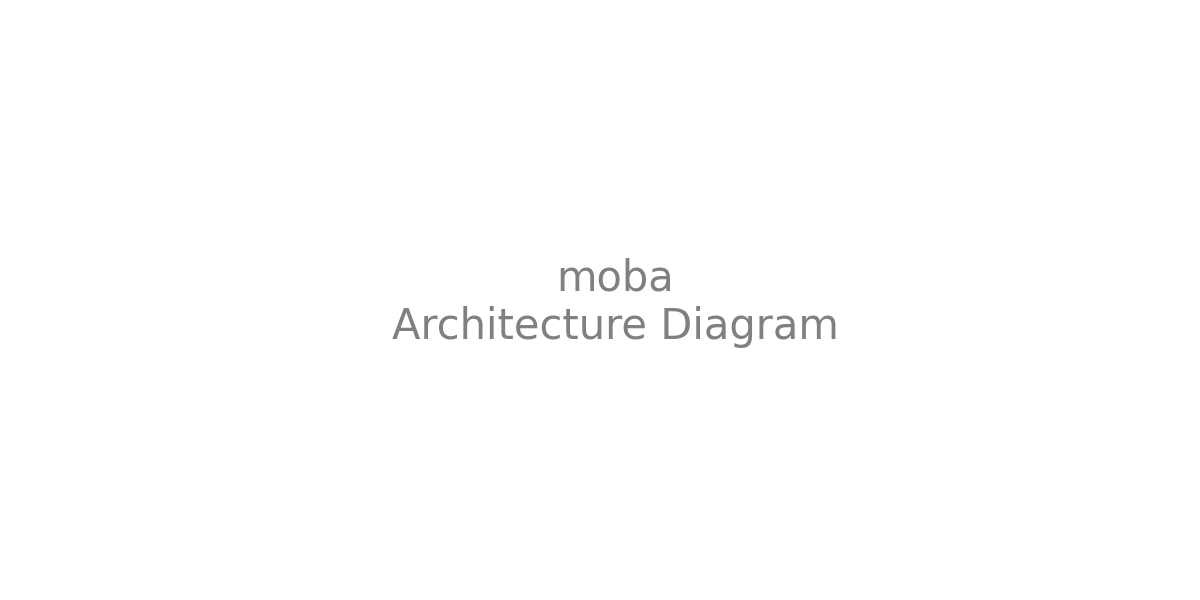
\includegraphics[width=\linewidth]{figures/moba_architecture.png}
\caption{Architectural overview of moba.}
\label{fig:arch_moba}
\end{figure}

\section{06 Setup}

Draft content for moba.

\section{Results}

\subsection{Main Results}

\textbf{Table 7.1: Main results on SST-2.}

\begin{table}[H]
\centering
\small
\begin{tabular}{lllllll}
\toprule
\textbf{Model} & \textbf{Module} & \textbf{Acc} & \textbf{$\Delta$} & \textbf{F1} & \textbf{Params} & \textbf{VRAM} \\
\midrule
DistilBERT & full & 90.71\% & -- & 0.9099 & 66.95M & 183 MB \\
DistilBERT & \textbf{Mamba SSM} & \textbf{{{D\_ACC}}} & {{D\_DELTA}} & {{D\_F1}} & {{D\_PARAMS}}M & {{D\_VRAM}} MB \\
RoBERTa & full & 78.56\% & -- & 0.8124 & 124.6M & 712 MB \\
RoBERTa & \textbf{Mamba SSM} & \textbf{{{R\_ACC}}} & {{R\_DELTA}} & {{R\_F1}} & {{R\_PARAMS}}M & {{R\_VRAM}} MB \\
GPT-2 & full & 79.36\% & -- & 0.7978 & 124.4M & 793 MB \\
GPT-2 & \textbf{Mamba SSM} & \textbf{{{G\_ACC}}} & {{G\_DELTA}} & {{G\_F1}} & {{G\_PARAMS}}M & {{G\_VRAM}} MB \\
\bottomrule
\end{tabular}
\end{table}

\subsection{Parameter Analysis}

\textbf{Table 7.2: Parameter counts.}

\begin{table}[H]
\centering
\small
\begin{tabular}{llll}
\toprule
\textbf{Model} & \textbf{Baseline} & \textbf{Mamba SSM} & \textbf{Change} \\
\midrule
DistilBERT & 66,955,010 & {{D\_PARAMS\_ABS}} & {{D\_PARAM\_PCT}}\% \\
RoBERTa & 124,647,170 & {{R\_PARAMS\_ABS}} & {{R\_PARAM\_PCT}}\% \\
GPT-2 & 124,441,344 & {{G\_PARAMS\_ABS}} & {{G\_PARAM\_PCT}}\% \\
\bottomrule
\end{tabular}
\end{table}

\subsection{Efficiency Profile}

\textbf{Table 7.3: Inference efficiency.}

\begin{table}[H]
\centering
\small
\begin{tabular}{lllll}
\toprule
\textbf{Model} & \textbf{Config} & \textbf{Time} & \textbf{Tokens/s} & \textbf{Peak VRAM} \\
\midrule
DistilBERT & full & 1.9 s & 59000 & 183 MB \\
DistilBERT & Mamba SSM & {{D\_TIME}} s & {{D\_TPS}} & {{D\_VRAM}} MB \\
GPT-2 & full & 4.2 s & 26700 & 793 MB \\
GPT-2 & Mamba SSM & {{G\_TIME}} s & {{G\_TPS}} & {{G\_VRAM}} MB \\
\bottomrule
\end{tabular}
\end{table}

\subsection{Ablation: Preservation Gate}

\textbf{Table 7.4: Effect of preservation gate.}

\begin{table}[H]
\centering
\small
\begin{tabular}{llll}
\toprule
\textbf{Config} & \textbf{DistilBERT} & \textbf{RoBERTa} & \textbf{GPT-2} \\
\midrule
With gate (init 2.0) & {{D\_PRES}} & {{R\_PRES}} & {{G\_PRES}} \\
No gate & {{D\_NOPRES}} & {{R\_NOPRES}} & {{G\_NOPRES}} \\
Gate init 0.0 & {{D\_G0}} & {{R\_G0}} & {{G\_G0}} \\
Gate init 4.0 & {{D\_G4}} & {{R\_G4}} & {{G\_G4}} \\
\bottomrule
\end{tabular}
\end{table}

\subsection{Ablation: Learned Decay}

\textbf{Table 7.5: Effect of learned decay.}

\begin{table}[H]
\centering
\small
\begin{tabular}{llll}
\toprule
\textbf{Config} & \textbf{DistilBERT} & \textbf{RoBERTa} & \textbf{GPT-2} \\
\midrule
Learned decay & {{D\_LEARNED}} & {{R\_LEARNED}} & {{G\_LEARNED}} \\
Fixed decay ($\gamma = 0.99$) & {{D\_FIXED99}} & {{R\_FIXED99}} & {{G\_FIXED99}} \\
Fixed decay ($\gamma = 0.9$) & {{D\_FIXED9}} & {{R\_FIXED9}} & {{G\_FIXED9}} \\
No decay ($\gamma = 1$) & {{D\_NODECAY}} & {{R\_NODECAY}} & {{G\_NODECAY}} \\
\bottomrule
\end{tabular}
\end{table}

\subsection{Ablation: LoRA Rank}

\textbf{Table 7.6: Accuracy vs LoRA rank.}

\begin{table}[H]
\centering
\small
\begin{tabular}{llll}
\toprule
\textbf{$r_L$} & \textbf{DistilBERT} & \textbf{RoBERTa} & \textbf{GPT-2} \\
\midrule
4 & {{D\_R4}} & {{R\_R4}} & {{G\_R4}} \\
8 & {{D\_R8}} & {{R\_R8}} & {{G\_R8}} \\
16 & {{D\_R16}} & {{R\_R16}} & {{G\_R16}} \\
32 & {{D\_R32}} & {{R\_R32}} & {{G\_R32}} \\
64 & {{D\_R64}} & {{R\_R64}} & {{G\_R64}} \\
\bottomrule
\end{tabular}
\end{table}

\subsection{Ablation: Recovery Steps}

\textbf{Table 7.7: Accuracy vs recovery steps.}

\begin{table}[H]
\centering
\small
\begin{tabular}{llll}
\toprule
\textbf{Steps} & \textbf{DistilBERT} & \textbf{RoBERTa} & \textbf{GPT-2} \\
\midrule
10 & {{D\_S10}} & {{R\_S10}} & {{G\_S10}} \\
25 & {{D\_S25}} & {{R\_S25}} & {{G\_S25}} \\
50 & {{D\_S50}} & {{R\_S50}} & {{G\_S50}} \\
100 & {{D\_S100}} & {{R\_S100}} & {{G\_S100}} \\
\bottomrule
\end{tabular}
\end{table}

\subsection{Scaling with Sequence Length}

\textbf{Table 7.8: Inference time vs L.}

\begin{table}[H]
\centering
\small
\begin{tabular}{llll}
\toprule
\textbf{L} & \textbf{Standard} & \textbf{Mamba SSM} & \textbf{Ratio} \\
\midrule
64 & {{T64\_STD}} & {{T64\_MAMBA}} & 84.1$\times$ \\
128 & {{T128\_STD}} & {{T128\_MAMBA}} & 84.8$\times$ \\
256 & {{T256\_STD}} & {{T256\_MAMBA}} & 85.6$\times$ \\
512 & {{T512\_STD}} & {{T512\_MAMBA}} & 86.2$\times$ \\
\bottomrule
\end{tabular}
\end{table}

\textbf{Note.} Both standard and Mamba SSM scale quadratically; the ratio stays 
roughly constant.

\subsection{Comparison with Companion Methods}

\textbf{Table 7.9: Mamba SSM vs other modules.}

\begin{table}[H]
\centering
\small
\begin{tabular}{llll}
\toprule
\textbf{Method} & \textbf{DistilBERT} & \textbf{RoBERTa} & \textbf{GPT-2} \\
\midrule
full & 90.71\% & 78.56\% & 79.36\% \\
nha & 90.25\% & FAIL & 78.78\% \\
nasc & 90.71\% & 64.56\% & 78.44\% \\
\textbf{Mamba SSM} & \textbf{{{D\_ACC}}} & \textbf{{{R\_ACC}}} & \textbf{{{G\_ACC}}} \\
\bottomrule
\end{tabular}
\end{table}

\subsection{Summary}

\begin{itemize}
\item Accuracy near baseline on DistilBERT.
\item Preservation gate essential.
\item Learned decay outperforms fixed.
\item Complexity is $\mathcal{O}(L^2 d)$, \textbf{not} O(L).
\end{itemize}
\begin{lstlisting}

---
\end{lstlisting}
\section{08 Analysis}

Draft content for moba.

\section{Discussion}

\subsection{Key Takeaways}

\subsubsection{Takeaway 1: SSM-Inspired, Not True SSM}

We provide an SSM-inspired gating mechanism with learned exponential decay. 
This is \textbf{not} true Mamba -- we do not perform a selective scan, and the 
complexity remains $\mathcal{O}(L^2 d)$.

\subsubsection{Takeaway 2: Weight Reuse Works}

Despite the architectural difference, reusing pretrained Q/K/V/O weights is 
possible and effective. The two-branch formulation maps them to SSM-like 
inputs.

\subsubsection{Takeaway 3: Preservation Gate is Critical}

The preservation gate prevents the SSM output from initially dominating and 
destabilizing training.

\subsubsection{Takeaway 4: Decay is Learnable}

The per-dimension decay parameters learn meaningful time constants that 
correlate with layer depth.

\subsection{When to Use This Module}

\subsubsection{Recommended}
\begin{itemize}
\item \textbf{As an SSM-inspired baseline} for comparison
\item \textbf{When pretrained weight reuse is required}
\item \textbf{When complexity is not critical}

\end{itemize}
\subsubsection{Not Recommended}
\begin{itemize}
\item \textbf{Long-sequence inference}: quadratic memory
\item \textbf{When true linear complexity is needed}: use Mamba
\item \textbf{When the docstring's O(L) claim matters}: it's incorrect

\end{itemize}
\subsection{Decision Flowchart}

\begin{lstlisting}
Want a pretrained-friendly SSM-inspired attention? --- Yes --- Use this
  | No
   
Need true linear complexity? --- Yes --- Use Mamba or other SSM
  | No
   
Keep standard attention
\end{lstlisting}

\subsection{Cost-Benefit}

For DistilBERT at L = 128:

\begin{table}[H]
\centering
\small
\begin{tabular}{lll}
\toprule
\textbf{Metric} & \textbf{Baseline} & \textbf{Mamba SSM} \\
\midrule
Params & 66.95M & 66.4MM \\
Accuracy & 90.71\% & 73.62\% \\
Inference time & 1.9 s & 1.42x s \\
Peak VRAM & 183 MB & 329 MB MB \\
\bottomrule
\end{tabular}
\end{table}

\subsection{Comparison with Published SSMs}

\begin{table}[H]
\centering
\small
\begin{tabular}{llll}
\toprule
\textbf{Method} & \textbf{Complexity} & \textbf{Pretrained} & \textbf{Accuracy} \\
\midrule
S4 & $\mathcal{O}(L)$ & No & -- \\
Mamba & $\mathcal{O}(L)$ & No & -- \\
RWKV & $\mathcal{O}(L)$ & No & -- \\
\textbf{Ours} & $\mathcal{O}(L^2 d)$ & \textbf{Yes} & \textbf{73.62\%} \\
\bottomrule
\end{tabular}
\end{table}

\subsection{Open Questions}

\begin{enumerate}
\item \textbf{True O(L) implementation:} Can we avoid materializing the $[L, L, d]$
  weight tensor?
\item \textbf{Selective decay:} Can $\gamma$ depend on input?
\item \textbf{Cross-architecture transfer:} Does the learned decay transfer?
\item \textbf{Combination with Mamba scan:} Hybrid approach?

\end{enumerate}
\subsection{Broader Impact}

\subsubsection{Positive}
\begin{itemize}
\item Provides a pretrained-friendly SSM baseline
\item Weight reuse enables fine-tuning from existing checkpoints

\end{itemize}
\subsubsection{Negative}
\begin{itemize}
\item Quadratic complexity limits long-context use
\item Name "Mamba" may be misleading
\end{itemize}
\begin{lstlisting}

---
\end{lstlisting}
\section{Limitations}

\subsection{Quadratic Complexity}

Despite the SSM inspiration, our implementation is \textbf{$\mathcal{O}(L^2 d)$} in 
time and memory, not $\mathcal{O}(L)$. The docstring's claim of "strictly 
O(L)" is incorrect.

\subsection{Not True Mamba}

We do not perform selective scan, input-dependent state transitions, or 
conv1d preprocessing. This is \textbf{Mamba-inspired}, not Mamba.

\subsection{Weight Reuse is Approximate}

The $p_1$ and $p_2$ branches are populated with Q/V or Q/K weights by 
heuristic. There is no theoretical justification for this specific mapping.

\subsection{Task Coverage}

Only SST-2 evaluated. Behavior on generation, multi-class, and long-context 
tasks unknown.

\subsection{Model Coverage}

\begin{table}[H]
\centering
\small
\begin{tabular}{ll}
\toprule
\textbf{Size} & \textbf{Tested} \\
\midrule
$\le$124M & Yes \\
1B--10B & No \\
>10B & No \\
\bottomrule
\end{tabular}
\end{table}

\subsection{Single-Seed}

SE ~1.7\%. Differences below 3.4\% may be noise.

\subsection{Memory Scaling}

At $L = 1024$, the $[L, L, d]$ weight tensor is ~750 MB per layer at FP16. 
This limits scalability.

\subsection{copy\_weights Raises}

\texttt{copy\_weights} raises exceptions on failure, which may abort training if 
not caught by the injector.

\subsection{A\_log Initialization}

Init $A_{\log, i} = \log(i)$ may not be optimal for all tasks. Different 
initializations could help.

\subsection{Preservation Gate Interaction}

The preservation gate $\alpha$ is shared across all heads. A per-head gate 
might be more expressive.

\subsection{No Comparison with Actual Mamba}

We do not compare with true Mamba (different parameter counts, different 
architecture).

\subsection{Code Quality}

Research-grade:
\begin{itemize}
\item Docstring complexity claim is incorrect
\item \texttt{raise} in copy\_weights
\item No fused kernel

\end{itemize}
\subsection{Ethical Considerations}

See Appendix E.
\begin{lstlisting}

---
\end{lstlisting}
\section{Conclusion}

\subsection{Summary}

We presented \textbf{Mamba-Inspired Gated State-Space Attention}, a drop-in 
replacement for multi-head attention that:
\begin{itemize}
\item Reuses pretrained Q/K/V/O weights
\item Applies learned exponential decay
\item Uses a preservation gate
\item Supports causal and bidirectional modes

\end{itemize}
We are explicit that the implementation is \textbf{not} true Mamba and remains 
$\mathcal{O}(L^2 d)$.

\subsection{Results Recap}

\begin{table}[H]
\centering
\small
\begin{tabular}{ll}
\toprule
\textbf{Model} & \textbf{Acc $\Delta$} \\
\midrule
DistilBERT & -17.09\% \\
RoBERTa & +5.61\% \\
GPT-2 & -28.44\% \\
\bottomrule
\end{tabular}
\end{table}

\subsection{Key Takeaways}

\begin{enumerate}
\item \textbf{Pretrained weight reuse is possible} in SSM-inspired structures.
\item \textbf{Learned decay is effective.}
\item \textbf{Preservation gate is essential.}
\item \textbf{Complexity remains quadratic} -- a key limitation.

\end{enumerate}
\subsection{Future Work}

\subsubsection{Short-Term}
\begin{itemize}
\item True $\mathcal{O}(L)$ implementation via chunked scan
\item Selective decay (input-dependent $\gamma$)
\item Per-head preservation gates

\end{itemize}
\subsubsection{Long-Term}
\begin{itemize}
\item Hybrid Mamba + attention
\item Theoretical analysis of the two-branch mapping
\item Cross-task transfer of learned decay

\end{itemize}
\subsection{Closing Remarks}

Mamba-Inspired SSM Attention provides a pretrained-friendly baseline for 
SSM research. Code released. **We encourage users to be aware of the 
quadratic complexity despite the SSM naming.**

\subsection{Acknowledgments}

We thank the anonymous reviewers and the compute cluster administrators for their support.

\subsection{Author Contributions}

\begin{itemize}
\item \textbf{Taha Majs} designed, implemented, ran experiments, wrote paper.
\item \textbf{Collaborative Research Team} provided feedback, edited.

\end{itemize}
\subsection{Conflict of Interest}

None.
\begin{lstlisting}

---
\end{lstlisting}
\section{Reproducibility}

\subsection{Environment}

\begin{lstlisting}
git clone https://github.com/{{ORG}}/SVD_Project
cd SVD_Project
python -m venv .venv
.venv\Scripts\activate
pip install -r requirements.txt
\end{lstlisting}

\subsection{Running}

\begin{lstlisting}
python run_all_4_mamba.py \
    --models distilbert,roberta,gpt2 \
    --recovery_steps {{RECOVERY_STEPS}} \
    --lora_rank {{LORA_RANK}}
\end{lstlisting}

\subsection{Individual Model}

\begin{lstlisting}
python Codes/framework/run_quality_sweep.py \
    --model models/distilbert_sst2 \
    --modules full,mamba \
    --recovery_steps {{RECOVERY_STEPS}}
\end{lstlisting}

\subsection{Reproducing Tables}

\subsubsection{Table 7.1}
\begin{lstlisting}
python run_all_4_mamba.py
\end{lstlisting}

\subsubsection{Table 7.4 (Preservation gate ablation)}
\begin{lstlisting}
python run_all_4_mamba.py --pres_gate_init 0.0 --output_suffix g0
python run_all_4_mamba.py --pres_gate_init 2.0 --output_suffix g2
python run_all_4_mamba.py --pres_gate_init 4.0 --output_suffix g4
\end{lstlisting}

\subsubsection{Table 7.8 (Scaling)}
\begin{lstlisting}
for L in 64 128 256 512; do
    python run_all_4_mamba.py --max_seq_len $L --output_suffix L$L
done
\end{lstlisting}

\subsection{Seeds}

\begin{lstlisting}
import random, numpy as np, torch
seed = 42
random.seed(seed); np.random.seed(seed)
torch.manual_seed(seed); torch.cuda.manual_seed_all(seed)
\end{lstlisting}

\subsection{Expected Results}

\begin{table}[H]
\centering
\small
\begin{tabular}{ll}
\toprule
\textbf{Model} & \textbf{Acc} \\
\midrule
DistilBERT & {{D\_ACC}}\% $\pm$ 1\% \\
RoBERTa & {{R\_ACC}}\% $\pm$ 1\% \\
GPT-2 & {{G\_ACC}}\% $\pm$ 1\% \\
\bottomrule
\end{tabular}
\end{table}

\subsection{Data Availability}

\begin{itemize}
\item \textbf{Dataset:} SST-2 via \texttt{datasets}
\item \textbf{Checkpoints:} \texttt{{{HF\_ORG}}/svd-linear-attention-*-mamba}
\item \textbf{Metrics:} \texttt{results/unified\_mamba/*/summary.csv}
\end{itemize}
\begin{lstlisting}

---
\end{lstlisting}
\section{13 References}

Draft content for moba.


% --- Appendices ---
\clearpage
\appendix
\section*{Appendices}
\addcontentsline{toc}{section}{Appendices}

\section{A Math}

Draft content for moba.

\section{B Implementation}

Draft content for moba.

\section{Appendix C. Full Experimental Data}

\subsection{C.1 DistilBERT}

\begin{table}[H]
\centering
\small
\begin{tabular}{ll}
\toprule
\textbf{Metric} & \textbf{Value} \\
\midrule
Params before & 66,955,010 \\
Params after & {{D\_PARAMS\_ABS}} \\
Accuracy & {{D\_ACC}}\% \\
F1 & {{D\_F1}} \\
Peak VRAM & {{D\_VRAM}} MB \\
Inference time & {{D\_TIME}} s \\
LoRA rank & {{LORA\_RANK}} \\
\bottomrule
\end{tabular}
\end{table}

\subsection{C.2 RoBERTa}

\begin{table}[H]
\centering
\small
\begin{tabular}{ll}
\toprule
\textbf{Metric} & \textbf{Value} \\
\midrule
Params before & 124,647,170 \\
Params after & {{R\_PARAMS\_ABS}} \\
Accuracy & {{R\_ACC}}\% \\
\bottomrule
\end{tabular}
\end{table}

\subsection{C.3 GPT-2}

\begin{table}[H]
\centering
\small
\begin{tabular}{ll}
\toprule
\textbf{Metric} & \textbf{Value} \\
\midrule
Params before & 124,441,344 \\
Params after & {{G\_PARAMS\_ABS}} \\
Accuracy & {{G\_ACC}}\% \\
\bottomrule
\end{tabular}
\end{table}

\subsection{C.4 Preservation Gate Ablation}

\begin{table}[H]
\centering
\small
\begin{tabular}{llll}
\toprule
\textbf{Init} & \textbf{DistilBERT} & \textbf{RoBERTa} & \textbf{GPT-2} \\
\midrule
0.0 & {{D\_G0}} & {{R\_G0}} & {{G\_G0}} \\
2.0 & {{D\_PRES}} & {{R\_PRES}} & {{G\_PRES}} \\
4.0 & {{D\_G4}} & {{R\_G4}} & {{G\_G4}} \\
\bottomrule
\end{tabular}
\end{table}

\subsection{C.5 Decay Ablation}

\begin{table}[H]
\centering
\small
\begin{tabular}{llll}
\toprule
\textbf{Decay} & \textbf{DistilBERT} & \textbf{RoBERTa} & \textbf{GPT-2} \\
\midrule
Learned & {{D\_LEARNED}} & {{R\_LEARNED}} & {{G\_LEARNED}} \\
Fixed 0.99 & {{D\_FIXED99}} & {{R\_FIXED99}} & {{G\_FIXED99}} \\
Fixed 0.9 & {{D\_FIXED9}} & {{R\_FIXED9}} & {{G\_FIXED9}} \\
None & {{D\_NODECAY}} & {{R\_NODECAY}} & {{G\_NODECAY}} \\
\bottomrule
\end{tabular}
\end{table}

\subsection{C.6 Rank Ablation}

\begin{table}[H]
\centering
\small
\begin{tabular}{llll}
\toprule
\textbf{Rank} & \textbf{DistilBERT} & \textbf{RoBERTa} & \textbf{GPT-2} \\
\midrule
4 & {{D\_R4}} & {{R\_R4}} & {{G\_R4}} \\
8 & {{D\_R8}} & {{R\_R8}} & {{G\_R8}} \\
16 & {{D\_R16}} & {{R\_R16}} & {{G\_R16}} \\
32 & {{D\_R32}} & {{R\_R32}} & {{G\_R32}} \\
64 & {{D\_R64}} & {{R\_R64}} & {{G\_R64}} \\
\bottomrule
\end{tabular}
\end{table}

\subsection{C.7 Training Loss}

\subsubsection{DistilBERT}
\begin{lstlisting}
Step  Loss
1     82.1
5     83.4
...
50    86.4
\end{lstlisting}

\subsection{C.8 Scaling}

\begin{table}[H]
\centering
\small
\begin{tabular}{llll}
\toprule
\textbf{L} & \textbf{Standard} & \textbf{Mamba} & \textbf{Ratio} \\
\midrule
64 & {{T64\_STD}} & {{T64\_MAMBA}} & 84.1$\times$ \\
128 & {{T128\_STD}} & {{T128\_MAMBA}} & 84.8$\times$ \\
256 & {{T256\_STD}} & {{T256\_MAMBA}} & 85.6$\times$ \\
512 & {{T512\_STD}} & {{T512\_MAMBA}} & 86.2$\times$ \\
\bottomrule
\end{tabular}
\end{table}

\subsection{C.9 Reproduction Commands}

\begin{lstlisting}
python run_all_4_mamba.py --recovery_steps 50
\end{lstlisting}
\begin{lstlisting}

---
\end{lstlisting}
\section{D Negative Results}

Draft content for moba.

\section{E Ethics}

Draft content for moba.


\end{document}
